\documentclass[10pt,paper=a5,pagesize]{scrbook}
\usepackage{geometry}
\usepackage{fontspec}                           
\usepackage{graphicx}
\usepackage{tcolorbox}
\usepackage[french]{babel}
\usepackage{tikz}
\usepackage{rubikcube,rubikrotation}
\usepackage{parskip}
\usepackage{enumitem}
\usepackage{pdfpages}
\usepackage{url}
\usepackage[nochapter]{vhistory}


\usetikzlibrary{arrows}
\setlist[itemize,1]{label={\fontfamily{cmr}\fontencoding{T1}\selectfont\textbullet}}

\setmainfont{Alegreya Sans}

\newfontfamily\barlow{Barlow Semi Condensed}
\setkomafont{disposition}{\barlow}

\begin{document}
\frontmatter
\thispagestyle{empty}

\begin{titlepage}
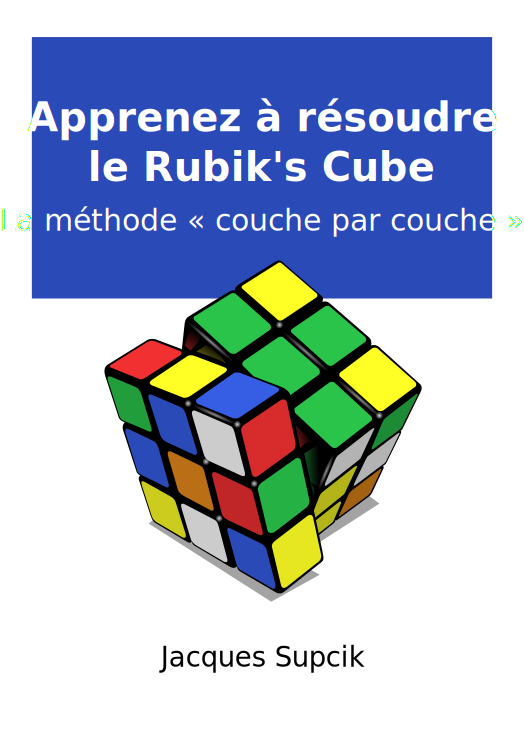
\includepdf{title}
\end{titlepage}

\thispagestyle{empty}
\null
\vfill

Le code source de ce document est disponible sur github à l'adresse\\
\url{https://github.com/supcik/manuel-rubik-cube-fr}.
\par\vspace*{8mm}

\begin{minipage}[c]{\textwidth}
\begin{versionhistory}
	\vhEntry{1.0.4}{7.03.2024}{JS}{Version HEIA-FR}
	\vhEntry{1.0.3}{5.06.2022}{JS}{Corrections mineures}
	\vhEntry{1.0.2}{20.06.2019}{JS}{Nouvelle page de titre}
	\vhEntry{1.0.1}{17.06.2019}{JS}{Corrections}
	\vhEntry{0.0.0}{20.02.2016}{JS}{Première ébauche}
\end{versionhistory}
\end{minipage}
\par\vspace*{10mm}


\includegraphics[width=30mm]{by.pdf}

Copyright \textcopyright{} 2024 Jacques Supcik

Cette œuvre est mise à disposition selon les termes de la Licence Creative Commons Attribution 4.0 International.
\medskip\\
Pour obtenir une copie de la licence, visitez:\\
\url{http://creativecommons.org/licenses/by/4.0/deed.fr}.
\newpage

\tableofcontents
\chapter*{Remerciements}

Merci à tous ceux qui ont contribué à la réalisation de ce livre. Merci à Pascal Supcik pour la relecture du manuscrit et la correction de nombreuses erreurs. Merci à Milena Supcik, Damien Goetschi et Baptiste Wicht pour avoir testé les méthodes lors des ateliers avec les enfants. Merci enfin à tous les enfants qui ont utilisé une première version de ce livre et qui m'ont permis d'améliorer certains passages.
\mainmatter
\chapter{Introduction}

Le Rubik's cube a été inventé en 1974 par le sculpteur et professeur d'architecture hongrois \emph{Ernő Rubik}. Pour la petite histoire, il a fallu plus d'un mois à Ernő Rubik pour résoudre sa propre invention! Ce cube était très populaire
dans les années~80, et aujourd'hui encore, il reste un objet très apprécié
par tous ceux qui s'intéressent aux sciences, aux mathématiques, ou à la technologie.

Les règles du jeu sont extrêmement simples: il suffit de faire pivoter les parties du cube de manière à rassembler toutes les pastilles de la même couleur sur la même face:

\begin{center}
	\RubikCubeSolved
	\ShowCube{2cm}{0.5}{%
		\DrawRubikCubeRU
	}
\end{center}


Mais la simplicité s'arrête là. En effet, il y a plus de 43~trillions\footnote{Pour être précis, il y a 43\,252\,003\,274\,489\,856\,000 configurations possibles.} configurations possibles du cube et il est très difficile de prévoir quels mouvements seront nécessaires pour résoudre un cube bien «mélangé».

Des chercheurs ont démontré\cite{god20} qu'on pouvait résoudre n'importe quel cube avec un maximum de 20~mouvements. La méthode \emph{couche par couche} présentée dans ce livre nécessite beaucoup plus que 20~mouvements, mais elle a l'avantage d'être bien adaptée aux débutants. Si, plus
tard, vous souhaitez battre des records de vitesse, vous devrez apprendre
d'autres méthodes; plus rapides, mais aussi plus difficiles à mémoriser.
 
Nous commencerons par positionner toutes les pièces de la couche du haut, ensuite nous positionnerons les pièces de la couche du milieu et nous terminerons par les pièces de la dernière
couche. Prenez le temps de bien exercer chaque couche avant de passer
à la suivante. Vous n'apprendrez pas plus vite en brûlant les étapes. Si vous utilisez ce livre dans le cadre d'une série d'ateliers, vous pouvez très bien faire trois
séances de une heure chacune. Vous étudierez alors une couche par séance et vous aurez du temps pour vous exercer entre les séances. 


\chapter{Les différentes parties du cube}

Commençons par étudier les différentes parties du Rubik's cube.

\section{Les centres}

Le cube se compose de 6 \textbf{centres} qui sont toujours placés de la même manière:

\begin{center}
	\RubikFaceUp%
	{X}{X}{X}%
	{X}{W}{X}%
	{X}{X}{X}
	\RubikFaceRight%
	{X}{X}{X}%
	{X}{G}{X}%
	{X}{X}{X}
	\RubikFaceFront%
	{X}{X}{X}%
	{X}{O}{X}%
	{X}{X}{X}
	\ShowCube{2cm}{0.5}{%
		\DrawRubikCubeRU
	}
\end{center}

Les centres sont identifiés par une \textbf{pastille}\footnote{La plupart des cubes du commerce ont des auto-collants pour identifier les couleurs.} de couleur. Les
couleurs du cube original sont blanc, rouge, bleu, orange, vert et jaune.
Si votre cube à d'autres couleurs ce n'est pas grave, la méthode reste la
même.

Les centres restent toujours à la même place; vous pouvez faire tous les mouvements que vous voulez, vous ne changerez jamais la position des centres.

\section{Les arrêtes}
\begin{samepage}
Le cube se compose également de 12 \textbf{arrêtes}:

\begin{center}
	\RubikFaceUp%
	{X}{W}{X}%
	{W}{X}{W}%
	{X}{W}{X}
	\RubikFaceRight%
	{X}{G}{X}%
	{G}{X}{G}%
	{X}{G}{X}
	\RubikFaceFront%
	{X}{O}{X}%
	{O}{X}{O}%
	{X}{O}{X}
	\ShowCube{2cm}{0.5}{%
		\DrawRubikCubeRU
	}
\end{center}
\end{samepage}

Les arrêtes sont les pièces placées entre les centres et elles ont toutes 2 pastilles de couleur. La deuxième couche du cube n'est composé que de quatre  centres et  quatre arrêtes.

\section{Les coins}

Pour terminer le cube a 8 \textbf{coins}:

\begin{center}
	\RubikFaceUp%
	{W}{X}{W}%
	{X}{X}{X}%
	{W}{X}{W}
	\RubikFaceRight%
	{G}{X}{G}%
	{X}{X}{X}%
	{G}{X}{G}
	\RubikFaceFront%
	{O}{X}{O}%
	{X}{X}{X}%
	{O}{X}{O}
	\ShowCube{2cm}{0.5}{%
		\DrawRubikCubeRU
	}
\end{center}

Chaque coin a 3 pastilles de couleur.

Il reste encore une pièce que nous ne voyons pas et qui est au milieu du cube. Si on additionne tous les types de pièces, on a $6 + 12 + 8 + 1 = 27$, ce qui correspond bien à ce que nous attendions avec un cube de $3 \times 3 \times 3$\footnote{$3 \cdot 3 \cdot 3 = 3^3 = 27$}.
\chapter{La première couche}

{
\centering
\RubikFaceUpAll{W}
\RubikFaceRight%
{G}{G}{G}%
{X}{G}{X}%
{X}{X}{X}
\RubikFaceFront%
{O}{O}{O}%
{X}{O}{X}%
{X}{X}{X}
\ShowCube{4cm}{1}{%
	\DrawRubikCubeRU
}
\par
}
\medskip

Pour commencer, nous allons résoudre la couche du haut du cube. Nous choisissons de positionner
le cube avec le centre blanc vers le haut, mais vous pouvez choisir une autre couleur si vous préférez.


\section{La croix}

Pour résoudre la première couche du cube, nous commençons
par faire une «croix» sur la face du haut.

\begin{center}
\RubikFaceUp%
{X}{W}{X}%
{W}{W}{W}%
{X}{W}{X}
\RubikFaceRight%
{X}{G}{X}%
{X}{G}{X}%
{X}{X}{X}
\RubikFaceFront%
{X}{O}{X}%
{X}{O}{X}%
{X}{X}{X}
\ShowCube{2cm}{0.5}{%
	\DrawRubikCubeRU
}
\end{center}

Notez qu'il ne suffit pas de mettre les 4~arêtes blanches sur la face du haut, il faut aussi
que l'autre côté des arêtes corresponde avec la couleur des autres centres (orange et vert dans l'exemple ci-dessus).

Cette première couche peut se résoudre de manière assez intuitive et certains n'auront pas besoin
d'aide. Voici cependant des indications pour ceux qui auraient plus de peine.

Notez que vous pouvez faire pivoter la couche du bas de votre cube tant que vous voulez sans «casser» ce que vous avez déjà fait sur les couches du haut. \rrh{D} ou \rrh{Dp}. Ça nous sera bien utile pour la suite.

\subsection{L'arête à déplacer se trouve sur la dernière couche}
\label{subsec:c1d}

Si l'arête que vous souhaitez déplacer pour faire la croix se trouve sur la couche du bas, vous pouvez tourner cette couche du bas pour l'amener sur la bonne face. Nous aurons alors deux cas possibles:

Soit l'arête à la face blanche vers le bas:

\begin{center}
	\RubikFaceDown%
	{X}{W}{X}%
	{X}{Y}{X}%
	{X}{X}{X}
	\RubikFaceRight%
	{X}{X}{X}%
	{X}{G}{X}%
	{X}{X}{X}
	\RubikFaceFront%
	{X}{X}{X}%
	{X}{O}{X}%
	{X}{O}{X}
	\ShowCube{2cm}{0.5}{%
		\DrawRubikCubeRD
	}
\end{center}

et dans ce cas, il suffit de faire tourner la face avant deux fois: \rrh{F}\rrh{F} (ou \rrh{Fp}\rrh{Fp}).

Ou alors l'arête blanche est sur la face avant:

\begin{center}
	\RubikFaceDown%
	{X}{O}{X}%
	{X}{Y}{X}%
	{X}{X}{X}
	\RubikFaceRight%
	{X}{X}{X}%
	{X}{G}{X}%
	{X}{X}{X}
	\RubikFaceFront%
	{X}{X}{X}%
	{X}{O}{X}%
	{X}{W}{X}
	\ShowCube{2cm}{0.5}{%
		\DrawRubikCubeRD
	}
\end{center}

Dans ce cas, nous faisons remonter l'arête avec les mouvements suivants: \rrh{D}\rrh{Sl}\rrh{Dp}\rrh{Slp}


\subsection{L'arête se trouve sur la couche du milieu}

Si l'arête se trouve sur la couche du milieu, comme ceci:

\begin{center}
	\RubikFaceUp%
	{X}{X}{X}%
	{X}{W}{X}%
	{X}{X}{X}
	\RubikFaceRight%
	{X}{X}{X}%
	{W}{G}{X}%
	{X}{X}{X}
	\RubikFaceFront%
	{X}{X}{X}%
	{X}{O}{O}%
	{X}{X}{X}
	\ShowCube{2cm}{0.5}{%
		\DrawRubikCubeRU
	}
\end{center}

On peut amener cette arête en place tout simplement en tournant la face avant dans le sens antihoraire\footnote{Dans le sens contraire des aiguilles d'une montre}: \rrh{Fp}.

Si l'arête se trouve sur la face du milieu, mais qu'elle est mal positionnée

\begin{center}
	\RubikFaceUp%
	{X}{X}{X}%
	{X}{W}{X}%
	{X}{X}{X}
	\RubikFaceRight%
	{X}{X}{X}%
	{O}{G}{X}%
	{X}{X}{X}
	\RubikFaceFront%
	{X}{X}{X}%
	{X}{O}{W}%
	{X}{X}{X}
	\ShowCube{2cm}{0.5}{%
		\DrawRubikCubeRU
	}
\end{center}

alors on peut déplace cette arête sur la couche du bas: \rrh{Rp}\rrh{Dp}\rrh{R} et on ramène l'arête correctement positionnée sur la couche du haut: \rrh{F}\rrh{F}


Si l'arête se trouve sur la couche du milieu, mais n'est pas sur la bonne face:

\begin{center}
	\RubikFaceUp%
	{X}{X}{X}%
	{X}{W}{X}%
	{X}{X}{X}
	\RubikFaceRight%
	{X}{X}{X}%
	{W}{R}{X}%
	{X}{X}{X}
	\RubikFaceFront%
	{X}{X}{X}%
	{X}{G}{O}%
	{X}{X}{X}
	\ShowCube{2cm}{0.5}{%
		\DrawRubikCubeRU
	}
\end{center}

alors on déplace cette arête sur la couche du bas: \rrh{F}\rrh{Dp}\rrh{Fp} et on applique la règle pour la couche du bas comme expliqué en \ref{subsec:c1d}.


Pour gagner du temps, lorsqu'on déplace une arête sur la couche du bas, on va positionner l'arête de manière à ce que sa face blanche soit vers le bas. C'est le cas pour l'exemple ci-dessus.

Si l'arête de positionnée comme dans le cube ci-dessous:

\begin{center}
	\RubikFaceUp%
	{X}{X}{X}%
	{X}{W}{X}%
	{X}{X}{X}
	\RubikFaceRight%
	{X}{X}{X}%
	{O}{R}{X}%
	{X}{X}{X}
	\RubikFaceFront%
	{X}{X}{X}%
	{X}{G}{W}%
	{X}{X}{X}
	\ShowCube{2cm}{0.5}{%
		\DrawRubikCubeRU
	}
\end{center}

Alors on fait: \rrh{Rp}\rrh{Dp}\rrh{R}

\subsection{L'arête se trouve sur la couche du haut}

Si l'arête se trouve sur la couche du haut, mais que ses couleurs sont inversées, comme dans l'exemple ci-dessous:

\begin{center}
	\RubikFaceUp%
	{X}{X}{X}%
	{X}{W}{X}%
	{X}{O}{X}
	\RubikFaceRight%
	{X}{X}{X}%
	{X}{G}{X}%
	{X}{X}{X}
	\RubikFaceFront%
	{X}{W}{X}%
	{X}{O}{X}%
	{X}{X}{X}
	\ShowCube{2cm}{0.5}{%
		\DrawRubikCubeRU
	}
\end{center}

On peut faire pivoter l'arête avec la séquence suivante: \rrh{F}\rrh{F}\rrh{D}\rrh{Sl}\rrh{Dp}\rrh{Slp}.

Les deux premiers mouvements mettent l'arête sur la dernière couche et la suite est la même séquence que dans la section \ref{subsec:c1d}.

\begin{samepage}
Si l'arête est déjà bien orientée, mais qu'elle n'est pas au bon endroit, comme dans l'exemple ci-dessous:

\begin{center}
	\RubikFaceUp%
	{X}{X}{X}%
	{X}{W}{W}%
	{X}{X}{X}
	\RubikFaceRight%
	{X}{O}{X}%
	{X}{G}{X}%
	{X}{X}{X}
	\RubikFaceFront%
	{X}{X}{X}%
	{X}{O}{X}%
	{X}{X}{X}
	\ShowCube{2cm}{0.5}{%
		\DrawRubikCubeRU
	}
\end{center}
\end{samepage}


Si c'est la première arête que vous mettez en place, vous pouvez simplement tourner la face du haut: \rrh{U}, mais si les autres arêtes sont déjà en place, vous pouvez alors amener l'arête sur la dernière couche: \rrh{Rp}\rrh{Rp}. L'arête se trouve alors sur la dernière couche et on applique la méthode expliquée en \ref{subsec:c1d}.

Si l'arête se trouve sur la dernière couche et qu'elle n'est ni bien orientée, ni bien positionnée:

\begin{center}
	\RubikFaceUp%
	{X}{X}{X}%
	{X}{W}{O}%
	{X}{X}{X}
	\RubikFaceRight%
	{X}{W}{X}%
	{X}{G}{X}%
	{X}{X}{X}
	\RubikFaceFront%
	{X}{X}{X}%
	{X}{O}{X}%
	{X}{X}{X}
	\ShowCube{2cm}{0.5}{%
		\DrawRubikCubeRU
	}
\end{center}

Vous pouvez l'amener sur la couche du bas: \rrh{Rp}\rrh{Rp}\rrh{Dp}\rrh{R}\rrh{R} et ensuite, appliquer la méthode expliquée en \ref{subsec:c1d}.

Notez que dans l'exemple ci-dessus, vous pouvez mettre l'arête en place en continuant avec la simple séquence suivante: \rrh{Rp}\rrh{Fp}

\section{Les coins de la première couche}

Pour terminer la première couche, il ne nous reste plus qu'à mettre les coins en place.

\subsection{Le coin à déplacer se trouve sur la couche du bas}
\label{subsec:c1cd}

Si le coin se trouve sur la dernière couche, il y a trois cas possibles.
Le premier cas est celui où le coin est placé avec le côté blanc vers
la face et il doit monter en diagonale: 

\begin{center}  	
	\RubikFaceRight%
	{X}{G}{X}%
	{X}{G}{X}%
	{X}{X}{X}
	\RubikFaceFront%
	{X}{O}{X}%
	{X}{O}{X}%
	{W}{X}{X}
	\RubikFaceDown%
	{G}{X}{X}%
	{X}{Y}{X}%
	{X}{X}{X}
	
	\ShowCube{2cm}{0.5}{%
	\DrawRubikCubeRD
	\tikzset{>=latex}
	\draw[thick,->] (0.5,0.5) -- (2.5,2.5);
	}
\end{center} 

On résout ce cas avec la séquence suivante:
\rrh{D}\rrh{D}\rrh{F}\rrh{Dp}\rrh{Fp}

Le deuxième cas est celui où le coin est placé avec le côté blanc vers
la face et il doit monter en vertical: 

\begin{center}
	\RubikFaceRight%
	{X}{G}{X}%
	{X}{G}{X}%
	{G}{X}{X}
	\RubikFaceFront%
	{X}{O}{X}%
	{X}{O}{X}%
	{X}{X}{W}
	\RubikFaceDown%
	{X}{X}{O}%
	{X}{Y}{X}%
	{X}{X}{X}
	
	\ShowCube{2cm}{0.5}{%
		\DrawRubikCubeRD
		\tikzset{>=latex}
		\draw[thick,->] (2.5,0.5) -- (2.5,2.5);
	}
\end{center} 

On résout ce cas avec la séquence suivante:
\rrh{Dp}\rrh{Rp}\rrh{D}\rrh{R}


Le troisième cas est celui où le coin est placé avec le côté blanc vers
le bas. On commence par placer le coin à la verticale de la position
vers laquelle on souhaite l'amener:

\begin{center}
	\RubikFaceRight%
	{X}{G}{X}%
	{X}{G}{X}%
	{O}{X}{X}
	\RubikFaceFront%
	{X}{O}{X}%
	{X}{O}{X}%
	{X}{X}{G}
	\RubikFaceDown%
	{X}{X}{W}%
	{X}{Y}{X}%
	{X}{X}{X}
	
	\ShowCube{2cm}{0.5}{%
		\DrawRubikCubeRD
		\tikzset{>=latex}
		\draw[thick,<->] (2.5,0.5) -- (2.5,2.5);
	}
\end{center} 

La séquence suivante permet de faire pivoter le coin et le mettre en bas à gauche: \rrh{Rp}\rrh{D}\rrh{D}\rrh{R}

\begin{samepage}
Le résultat sera:

\begin{center}
	\RubikFaceRight%
	{X}{G}{X}%
	{X}{G}{X}%
	{X}{X}{X}
	\RubikFaceFront%
	{X}{O}{X}%
	{X}{O}{X}%
	{W}{X}{X}
	\RubikFaceDown%
	{G}{X}{X}%
	{X}{Y}{X}%
	{X}{X}{X}
	
	\ShowCube{2cm}{0.5}{%
		\DrawRubikCubeRD
	}
\end{center} 
\end{samepage}
	
Ce qui correspond à un cas connu et nous savons alors comment le faire
venir à sa position finale.

\subsection{Le coin à déplacer se trouve sur la face du haut}

Les coins peuvent déjà se trouver soit sur la couche du haut, mais leur
position n'est peut-être pas la bonne.

Pour déplacer un coin, nous devons commencer par l'amener sur la couche du bas. Prenons l'exemple du cube ci-dessous:

\begin{center}
	\RubikFaceUp%
	{X}{W}{X}%
	{W}{W}{W}%
	{X}{W}{G}
	\RubikFaceRight%
	{O}{R}{X}%
	{X}{R}{X}%
	{X}{X}{X}
	\RubikFaceFront%
	{X}{G}{W}%
	{X}{G}{X}%
	{X}{X}{X}
	\ShowCube{2cm}{0.5}{%
		\DrawRubikCubeRU
	}
\end{center}

Nous avons 4~possibilités pour faire descendre ce coin sur la dernière couche:

\begin{itemize}
	\item \rrh{F}\rrh{D}\rrh{Fp}
	\item \rrh{F}\rrh{Dp}\rrh{Fp}
	\item \rrh{Rp}\rrh{D}\rrh{R}
	\item \rrh{Rp}\rrh{Dp}\rrh{R}		
\end{itemize}

Comme nous avons vu en \ref{subsec:c1cd}, c'est plus rapide si la face blanche du coin \textbf{n'est pas} dirigée vers le bas.

\begin{samepage}
Dans le cas ci-dessus, nous choisirons plutôt les variantes 1 et 3 qui se terminent avec les cubes suivants:

\begin{center}	
	\RubikFaceRight%
	{X}{R}{X}%
	{X}{R}{X}%
	{X}{X}{W}
	\RubikFaceFront%
	{X}{G}{X}%
	{X}{G}{X}%
	{X}{X}{X}
	\RubikFaceDown%
	{X}{X}{X}%
	{X}{Y}{X}%
	{X}{X}{O}
	\ShowCube{2cm}{0.5}{%
		\DrawRubikCubeRD
	}%
	\hspace*{1cm} 	
	\RubikFaceRight%
	{X}{R}{X}%
	{X}{R}{X}%
	{G}{X}{X}
	\RubikFaceFront%
	{X}{G}{X}%
	{X}{G}{X}%
	{X}{X}{W}
	\RubikFaceDown%
	{X}{X}{O}%
	{X}{Y}{X}%
	{X}{X}{X}
	\ShowCube{2cm}{0.5}{%
		\DrawRubikCubeRD
	}
\end{center} 
\end{samepage}
	
On pourrait bien aussi avoir le cas où le coin est bien placé, mais mal orienté:

\begin{center}
	\RubikFaceUp%
	{X}{W}{X}%
	{W}{W}{W}%
	{X}{W}{O}
	\RubikFaceRight%
	{W}{G}{X}%
	{X}{G}{X}%
	{X}{X}{X}
	\RubikFaceFront%
	{X}{O}{G}%
	{X}{O}{X}%
	{X}{X}{X}
	\ShowCube{2cm}{0.5}{%
		\DrawRubikCubeRU
	}
\end{center}

Dans ce cas également nous l'amènerons sur la couche du bas, par exemple avec \rrh{Rp}\rrh{Dp}\rrh{R}.
 
Ce qui donne:
 
\begin{center}
    \RubikFaceRight%
 	{X}{G}{X}%
 	{X}{G}{X}%
 	{X}{X}{X}
 	\RubikFaceFront%
 	{X}{O}{X}%
 	{X}{O}{X}%
 	{W}{X}{X}
 	\RubikFaceDown%
 	{G}{X}{X}%
 	{X}{Y}{X}%
 	{X}{X}{X}
 	\ShowCube{2cm}{0.5}{%
 		\DrawRubikCubeRD
 	}
\end{center} 


Ce cas est connu est nous savons comment faire monter ce coin en diagonale.

Voilà, vous avez maintenant toutes les informations pour résoudre la première
couche du cube. Entraînez-vous plusieurs fois à faire cette couche.

\chapter{La couche du milieu}

{
	\centering
	\RubikFaceUpAll{W}
	\RubikFaceRight%
	{G}{G}{G}%
	{G}{G}{G}%
	{X}{X}{X}
	\RubikFaceFront%
	{O}{O}{O}%
	{O}{O}{O}%
	{X}{X}{X}
	\ShowCube{4cm}{1}{%
		\DrawRubikCubeRU
	}
	\par
}
\medskip

Contrairement à la première couche, il est beaucoup plus difficile d'imaginer les mouvements qui permettent de positionner les arêtes de la deuxième couche. Nous devons alors apprendre une série de mouvements par cœur. Ça semble difficile, mais nous allons raconter une histoire, en relation avec les mouvements du cube, qui nous permettra de mieux mémoriser les mouvements. Par la suite, avec un peu de pratique, vous ferez ces séries de mouvements de manière automatique et vous n'aurez probablement plus besoin de l'histoire.  

L'histoire que nous utilisons pour mémoriser les mouvements est connue sous \og{}l'histoire du Belge\fg{}. Mais comme nous aimons bien les Belges et que nous ne voulons pas de problème avec eux, nous pouvons aussi dire que c'est \og{}l'histoire du distrait\fg{}.

\section{L'arête de trouve sur la couche du bas}\label{subsec:c21}

Si l'arête que nous souhaitons mettre en place se trouve sur la couche du bas, nous commençons par positionner cette arête en faisant correspondre la couleur de l'arête avec la couleur du centre. Nous avons alors 2 cas possibles. Le premier, c'est que l'arête doit \og{}monter\fg{} vers la \textbf{droite}:
\smallskip

\begin{center}
	\RubikFaceDown%
	{X}{G}{X}%
	{X}{Y}{X}%
	{X}{X}{X}
	\RubikFaceRight%
	{G}{G}{G}%
	{X}{G}{X}%
	{X}{X}{X}
	\RubikFaceFront%
	{O}{O}{O}%
	{X}{O}{X}%
	{X}{O}{X}
	\ShowCube{2cm}{0.5}{%
		\DrawRubikCubeRD
	\tikzset{>=latex}
	\draw[thick,->] (1.5,0.5) -- (2.5,1.5);	
	}
\end{center}
\smallskip

Voici l'\og{}histoire\fg{} qui permet de résoudre ce cas:
\begin{itemize}
	\item Il doit aller à droite, mais il se trompe et part à gauche: \rrh{Dp}.
	\item Ses amis viennent le chercher: \rrh{Rp}.
	\item Il se dirige alors dans le bon sens: \rrh{D}.
	\item Ses amis rentrent chez eux: \rrh{R}.
	\item Emporté par son élan, il continue trop loin: \rrh{D}.
	\item Il va tellement vite qu'il emporte la face avant: \rrh{F}.
	\item Il remarque enfin son erreur et retourne sur ses pas: \rrh{Dp}.
	\item La face avant peut se remettre en place: \rrh{Fp}.
\end{itemize}

Vous pouvez aussi vous amuser à ajouter des détails à l'histoire ou même à vous inventer votre propre histoire si ça vous aide. 

\newpage
Le deuxième cas c'est que l'arête doit \og{}monter\fg{} vers la \textbf{gauche}:
\smallskip

\begin{center}
	\RubikFaceDown%
	{X}{B}{X}%
	{X}{Y}{X}%
	{X}{X}{X}
	\RubikFaceLeft%
	{B}{B}{B}%
	{X}{B}{X}%
	{X}{X}{X}
	\RubikFaceFront%
	{O}{O}{O}%
	{X}{O}{X}%
	{X}{O}{X}
	\ShowCube{2cm}{0.5}{%
		\DrawRubikCubeLD
		\tikzset{>=latex}
		\draw[thick,->] (1.5,0.5) -- (0.5,1.5);	
	}
\end{center}
\smallskip

L'histoire est la même, mais le sens est inversé:
\begin{itemize}
	\item Il doit aller à gauche, mais il se trompe et part à droite: \rrh{D}.
	\item Ses amis viennent le chercher: \rrh{L}.
	\item Il se dirige alors dans le bon sens: \rrh{Dp}.
	\item Ses amis rentrent chez eux: \rrh{Lp}.
	\item Emporté par son élan, il continue trop loin: \rrh{Dp}.
	\item Il va tellement vite qu'il emporte la face avant: \rrh{Fp}.
	\item Il remarque enfin son erreur et retourne sur ses pas: \rrh{D}.
	\item La face avant peut se remettre en place: \rrh{F}.
\end{itemize}

\newpage
\section{L'arête de trouve sur la couche du milieu}

Si l'arête se trouve sur la couche du milieu, mais qu'elle n'est pas bien placée:
\smallskip

\begin{center}
	
	\RubikFaceUp%
	{W}{W}{W}%
	{W}{W}{W}%
	{W}{W}{W}
	\RubikFaceRight%
	{G}{G}{G}%
	{R}{G}{X}%
	{X}{X}{X}
	\RubikFaceFront%
	{O}{O}{O}%
	{X}{O}{B}%
	{X}{X}{X}
	\ShowCube{2cm}{0.5}{%
		\DrawRubikCubeRU
	}%
	\hspace*{5mm}ou\hspace*{3mm} 	
	\RubikFaceUp%
	{W}{W}{W}%
	{W}{W}{W}%
	{W}{W}{W}
	\RubikFaceRight%
	{G}{G}{G}%
	{O}{G}{X}%
	{X}{X}{X}
	\RubikFaceFront%
	{O}{O}{O}%
	{X}{O}{G}%
	{X}{X}{X}
	\ShowCube{2cm}{0.5}{%
		\DrawRubikCubeRU
	}
\end{center}
\smallskip

Il suffit de remplacer cette arête par n'importe laquelle de la couche du bas à l'aide de la séquence ci-dessus. L'arête remplacée se retrouvera sur la couche du bas et vous pourrez faire comme expliqué en \ref{subsec:c21}.

\smallskip
\begin{center}	
	\RubikFaceUp%
	{W}{W}{W}%
	{W}{W}{W}%
	{W}{W}{W}
	\RubikFaceRight%
	{G}{G}{G}%
	{X}{G}{X}%
	{X}{X}{X}
	\RubikFaceFront%
	{O}{O}{O}%
	{X}{O}{X}%
	{X}{X}{X}
	\ShowCube{2cm}{0.5}{%
		\DrawRubikCubeRU
	\tikzset{>=latex}
	\draw[thick,->] (1.5,0.5) -- (2.5,1.5);	
	}
\end{center}
\smallskip

C'est déjà tout pour la couche du milieu. Il vous suffit d'apprendre une histoire par cœur et de vous entraîner.

\chapter{La dernière couche}


{
	\centering
	\RubikFaceUpAll{W}
	\RubikFaceRight%
	{G}{G}{G}%
	{G}{G}{G}%
	{G}{G}{G}
	\RubikFaceFront%
	{O}{O}{O}%
	{O}{O}{O}%
	{O}{O}{O}
	\ShowCube{4cm}{1}{%
		\DrawRubikCubeRU
	}
	\par
}

Pour la dernière couche, nous retournons le cube. Si nous avons commencé avec la face blanche, ça veut dire que nous aurons la face jaune vers le haut. 

\section{La Croix}

Comme pour la première couche, nous commençons par réaliser une croix jaune.

\subsection{Une ligne sur la face}

\begin{samepage}
S’il y a une ligne jaune sur le cube, placez la ligne horizontalement comme sur la figure ci-dessous:

\begin{center}	
	\RubikFaceUp%
	{X}{X}{X}%
	{Y}{Y}{Y}%
	{X}{X}{X}
	\RubikFaceRight%
	{X}{X}{X}%
	{X}{B}{X}%
	{X}{X}{X}
	\RubikFaceFront%
	{X}{X}{X}%
	{X}{O}{X}%
	{X}{X}{X}
	\ShowCube{2cm}{0.5}{%
		\DrawRubikCubeRU
	}
\end{center}
\end{samepage}
	
Pour réaliser la croix à partir de cette position, faites la séquence de mouvements suivants:

\rrh{F}\rrh{R}\rrh{U}\rrh{Rp}\rrh{Up}\rrh{Fp}

Pour mémoriser cette suite de mouvements, vous pouvez inventer votre propre histoire. En voici une qui peut vous aider à trouver l'inspiration:

\begin{itemize}
	\item Il va dans le futur en fusée: \rrh{F}.
	\item Les extra-terrestres montent le voir: \rrh{R}.
	\item Il s'enfuit hors de la fusée: \rrh{U}.
	\item Les extra-terrestres rentrent chez eux: \rrh{Rp}.
	\item Il rentre dans la fusée: \rrh{Up}.
	\item Il revient dans le présent: \rrh{Fp}.
\end{itemize}

\subsection{Un «L» sur la face}
\begin{samepage}
Si au lieu d'une ligne, vous avez un «L» inversé sur la face:

\begin{center}	
	\RubikFaceUp%
	{X}{Y}{X}%
	{Y}{Y}{X}%
	{X}{X}{X}
	\RubikFaceRight%
	{X}{X}{X}%
	{X}{B}{X}%
	{X}{X}{X}
	\RubikFaceFront%
	{X}{X}{X}%
	{X}{O}{X}%
	{X}{X}{X}
	\ShowCube{2cm}{0.5}{%
		\DrawRubikCubeRU
	}
\end{center}
\end{samepage}
	
Vous pouvez obtenir une croix avec la séquence suivante:

\rrh{F}\rrh{U}\rrh{R}\rrh{Up}\rrh{Rp}\rrh{Fp}

Voici une histoire pour vous aider à mémoriser cette séquence.

\begin{itemize}
	\item Il va dans le futur: \rrh{F}.
	\item Il ouvre une boîte: \rrh{U}.
	\item Il en sort un billet: \rrh{R}.
	\item Il referme la boîte: \rrh{Up}.
	\item Il met le billet sans sa poche: \rrh{Rp}.
	\item Il revient dans le présent: \rrh{Fp}.
\end{itemize}

Vous pouvez bien évidemment inventer votre propre histoire si vous voulez.

\subsection{Autre configuration}

Si vous n'avez ni ligne ni «L» inversé, vous pouvez faire l'une ou l'autre des méthodes ci-dessus pour obtenir une configuration connue.

\section{Positionnement des arêtes}

Après avoir fait la croix, il est très probable que les arêtes ne soient pas bien positionnées. La séquence que nous allons voir permet de faire \textit{tourner} les trois arêtes comme dans la figure ci-dessous. Observez bien votre cube, positionnez la dernière couche pour faire correspondre l'arête avec le centre devant vous:

\begin{center}	
	\RubikFaceUp%
	{X}{Y}{X}%
	{Y}{Y}{Y}%
	{X}{Y}{X}
	\RubikFaceRight%
	{X}{G}{X}%
	{X}{B}{X}%
	{X}{X}{X}
	\RubikFaceFront%
	{X}{O}{X}%
	{X}{O}{X}%
	{X}{X}{X}
	\ShowCube{2cm}{0.5}{%
		\DrawRubikCubeRU
	}
\end{center}

Regardez si la rotation des arêtes comme montrée sur la figure suivante permet de bien positionner les arêtes. 
 

\begin{center}	
\ShowCube{2.1cm}{0.7}{%
	\DrawRubikLayerFace
	{X}{Y}{X}
	{Y}{Y}{Y}
	{X}{Y}{X}
	\tikzset{>=latex}
	\draw[thick,->] (2.5,1.5) -- (0.5,1.5);	
	\draw[thick,->] (0.5,1.5) -- (1.5,2.5);	
	\draw[thick,->] (1.5,2.5) -- (2.5,1.5);	
}
\end{center}

Si la couleur que vous avez choisie ne «fonctionne» pas, essayez avec une autre couleur. Si aucune couleur ne fonctionne, choisissez une couleur au hasard.

Pour faire tourner les arêtes comme indiqué sur la figure ci-dessus, nous utilisons \textbf{l'histoire de la chaise}:

\begin{itemize}
	\item Il se lève: \rrh{R}.
	\item Il part très très loin: \rrh{U}\rrh{U}.
	\item Sa chaise tombe: \rrh{Rp}.
	\item Il revient sur ses pas: \rrh{Up}.
	\item Il relève sa chaise: \rrh{R}.
	\item Il revient encore un peu plus sur ses pas: \rrh{Up}.	
	\item Il s'assied: \rrh{Rp}.
\end{itemize}

\section{Positionnement des sommets}

Une fois la croix terminée, nous allons positionner les 4 derniers sommets. Le but pour l'instant est de mettre les sommets au bon endroit, sans s'inquiéter de leurs orientations. Dans la figure ci-dessous, le sommet jaune-orange-bleu est bien placé.

\begin{center}	
	\RubikFaceUp%
	{X}{Y}{X}%
	{Y}{Y}{Y}%
	{X}{Y}{B}
	\RubikFaceRight%
	{O}{B}{X}%
	{X}{B}{X}%
	{X}{X}{X}
	\RubikFaceFront%
	{X}{O}{Y}%
	{X}{O}{X}%
	{X}{X}{X}
	\ShowCube{2cm}{0.5}{%
		\DrawRubikCubeRU
	}
\end{center}

Cherchez un sommet qui est déjà bien placé et mettez-le en haut à droite comme sur la figure ci-dessous. Nous faisons tourner les trois autres sommets avec l'histoire \textbf{des amis}:

\begin{itemize}
	\item Ses amis de gauche montent le voir: \rrh{Lp}.
	\item Il va les saluer:  \rrh{U}.
	\item Ses amis de droite montent le voir: \rrh{R}.
	\item Il va les saluer: \rrh{Up}.
	\item Ses amis de gauche se sentent seuls et descendent chez eux: \rrh{L}.
	\item Il va leur dire au revoir: \rrh{U}.
	\item Ses amis de droite se sentent seuls et descendent chez eux: \rrh{Rp}.
	\item Il va leur dire au revoir: \rrh{Up}.
\end{itemize}

Répétez cette séquence jusqu'à ce que les sommets soient tous bien placés.

\section{Orientation des sommets}

Pour terminer le cube, nous devons encore orienter les sommets. Avec la dernière séquence, nous pouvons faire pivoter les sommets comme indiqué sur la figure ci-dessous:

\begin{center}	
	\RubikFaceUp%
	{X}{Y}{B}%
	{Y}{Y}{Y}%
	{X}{Y}{B}
	\RubikFaceRight%
	{Y}{B}{Y}%
	{X}{B}{X}%
	{X}{X}{X}
	\RubikFaceFront%
	{X}{O}{O}%
	{X}{O}{X}%
	{X}{X}{X}
	\ShowCube{2cm}{0.5}{%
		\DrawRubikCubeRU
	\tikzset{>=latex}
	\draw[->] (3 + 1/6,2.5+0/6) -- (3 + 1/6,2.5+3/6);
	\draw[white,->] (3 + 0/6,2.5+4/6) -- (2.5 + 0/6,2.5+4/6);
	
	\draw[->] (3.5 + 2/6,3.0+1/6) -- (3.5 + 2/6,3.0+4/6);
	\draw[white,->] (3.5 + 1/6,3.0+5/6) -- (3.0 + 1/6,3.0+5/6);	
}
\end{center}

La séquence semble compliquée, mais c'est deux fois l'histoire de la chaise. Une première fois à droite:

\rrh{R}\rrh{U}\rrh{U}\rrh{Rp}\rrh{Up}\rrh{R}\rrh{Up}\rrh{Rp}

\begin{itemize}
	\item Il se lève: \rrh{R}.
	\item Il part très très loin: \rrh{U}\rrh{U}.
	\item Sa chaise tombe: \rrh{Rp}.
	\item Il revient sur ses pas: \rrh{Up}.
	\item Il relève sa chaise: \rrh{R}.
	\item Il revient encore un peu plus sur ses pas: \rrh{Up}.	
	\item Il s'assied: \rrh{Rp}.
\end{itemize}

Et une deuxième fois à gauche:

\rrh{Lp}\rrh{Up}\rrh{Up}\rrh{L}\rrh{U}\rrh{Lp}\rrh{U}\rrh{L}

\begin{itemize}
	\item Il se lève: \rrh{Lp}.
	\item Il part très très loin: \rrh{Up}\rrh{Up}.
	\item Sa chaise tombe: \rrh{L}.
	\item Il revient sur ses pas: \rrh{U}.
	\item Il relève sa chaise: \rrh{Lp}.
	\item Il revient encore un peu plus sur ses pas: \rrh{U}.	
	\item Il s'assied: \rrh{L}.
\end{itemize}

Répétez cette séquence tant que le cube n'est pas terminé.

\chapter{Notation}
La littérature sur le Rubik's cube utilise souvent une notation spécifique pour décrire les mouvements. La table de la page suivante décrit la notation la plus souvent utilisée.

Les lettres correspondent à la description de la face (en anglais): \textbf{R}ight (droit), \textbf{L}eft (gauche), \textbf{U}p (dessus), \textbf{D}own (dessous), \textbf{F}ront (avant), \textbf{B}ack (arrière).
Si la lettre est seule, il faut tourner dans le sens des aiguilles d'une montre.
Si la lettre est suivie d'un prime (') alors il faut tourner dans le sens \textbf{contraire} des aiguilles d'une montre. Si la lettre est suivie du chiffre 2, il faut répéter deux fois le mouvement (ce qui revient à lui faire faire un demi-tour, et le sens de rotation est donc égal).

Cette notation est également utilisée dans les concours pour indiquer comment \emph{mélanger} un cube\cite{scramble}. En partant du cube terminé, faites la séquence suivante:

\textbf{L2 U' B2 U2 B' -- U B U' L' F' -- L2 B D R D2 -- B2 F2 R' U L2 -- F2 D2 R B F}

Le résultat sera:

\begin{center}
	\RubikFaceRight%
	{R}{R}{W}%
	{G}{G}{R}%
	{O}{R}{O}
	\RubikFaceFront%
	{O}{O}{G}%
	{O}{O}{O}%
	{B}{Y}{W}
	\RubikFaceUp%
	{G}{B}{B}%
	{G}{W}{W}%
	{B}{Y}{W}
	\ShowCube{2cm}{0.5}{%
		\DrawRubikCubeRU
	}
\end{center} 

\setlength{\tabcolsep}{8pt}
\begin{center}
\begin{tabular}{ccccc}
{\Huge\textbf{R}} &
\RubikFaceRight%
{X}{X}{X}%
{X}{X}{X}%
{X}{X}{X}
\RubikFaceFront%
{X}{X}{B}%
{X}{X}{B}%
{X}{X}{B}
\RubikFaceUp%
{X}{X}{B}%
{X}{X}{B}%
{X}{X}{B}
\ShowCube{2cm}{0.5}{%
	\DrawRubikCubeRU
	\tikzset{>=latex}
	\draw[red, thick,->] (2.5,0.5) -- (2.5,3) -- (2.5+5/6,3+5/6);
}
& \hspace*{5mm} &
{\Huge\textbf{R'}} &
\RubikFaceRight%
{X}{X}{X}%
{X}{X}{X}%
{X}{X}{X}
\RubikFaceFront%
{X}{X}{B}%
{X}{X}{B}%
{X}{X}{B}
\RubikFaceUp%
{X}{X}{B}%
{X}{X}{B}%
{X}{X}{B}
\ShowCube{2cm}{0.5}{%
	\DrawRubikCubeRU
	\tikzset{>=latex}
	\draw[red, thick,<-] (2.5,0.5) -- (2.5,3) -- (2.5+5/6,3+5/6);
}
\\
\noalign{\medskip}
{\Huge\textbf{L}} &

\RubikFaceRight%
{X}{X}{X}%
{X}{X}{X}%
{X}{X}{X}
\RubikFaceFront%
{B}{X}{X}%
{B}{X}{X}%
{B}{X}{X}
\RubikFaceUp%
{B}{X}{X}%
{B}{X}{X}%
{B}{X}{X}
\ShowCube{2cm}{0.5}{%
	\DrawRubikCubeRU
	\tikzset{>=latex}
	\draw[red, thick,<-] (0.5,0.5) -- (0.5,3) -- (0.5+5/6,3+5/6);
}
& \hspace*{5mm} &
{\Huge\textbf{L'}} &
\RubikFaceRight%
{X}{X}{X}%
{X}{X}{X}%
{X}{X}{X}
\RubikFaceFront%
{B}{X}{X}%
{B}{X}{X}%
{B}{X}{X}
\RubikFaceUp%
{B}{X}{X}%
{B}{X}{X}%
{B}{X}{X}
\ShowCube{2cm}{0.5}{%
	\DrawRubikCubeRU
	\tikzset{>=latex}
	\draw[red, thick,->] (0.5,0.5) -- (0.5,3) -- (0.5+5/6,3+5/6);
}
\\
\noalign{\medskip}
{\Huge\textbf{U}} &
\RubikFaceRight%
{B}{B}{B}%
{X}{X}{X}%
{X}{X}{X}
\RubikFaceFront%
{B}{B}{B}%
{X}{X}{X}%
{X}{X}{X}
\RubikFaceUp%
{X}{X}{X}%
{X}{X}{X}%
{X}{X}{X}
\ShowCube{2cm}{0.5}{%
	\DrawRubikCubeRU
	\tikzset{>=latex}
	\draw[red, thick,<-] (0.5,2.5) -- (3,2.5) -- (3+5/6,2.5+5/6);
}
& \hspace*{5mm} &
{\Huge\textbf{U'}} &
\RubikFaceRight%
{B}{B}{B}%
{X}{X}{X}%
{X}{X}{X}
\RubikFaceFront%
{B}{B}{B}%
{X}{X}{X}%
{X}{X}{X}
\RubikFaceUp%
{X}{X}{X}%
{X}{X}{X}%
{X}{X}{X}
\ShowCube{2cm}{0.5}{%
	\DrawRubikCubeRU
	\tikzset{>=latex}
	\draw[red, thick,->] (0.5,2.5) -- (3,2.5) -- (3+5/6,2.5+5/6);
}
\\
\noalign{\medskip}
{\Huge\textbf{D}} &
\RubikFaceRight%
{X}{X}{X}%
{X}{X}{X}%
{B}{B}{B}
\RubikFaceFront%
{X}{X}{X}%
{X}{X}{X}%
{B}{B}{B}
\RubikFaceUp%
{X}{X}{X}%
{X}{X}{X}%
{X}{X}{X}
\ShowCube{2cm}{0.5}{%
	\DrawRubikCubeRU
	\tikzset{>=latex}
	\draw[red, thick,->] (0.5,0.5) -- (3,0.5) -- (3+5/6,0.5+5/6);
}
& \hspace*{5mm} &
{\Huge\textbf{D'}} &
\RubikFaceRight%
{X}{X}{X}%
{X}{X}{X}%
{B}{B}{B}
\RubikFaceFront%
{X}{X}{X}%
{X}{X}{X}%
{B}{B}{B}
\RubikFaceUp%
{X}{X}{X}%
{X}{X}{X}%
{X}{X}{X}
\ShowCube{2cm}{0.5}{%
	\DrawRubikCubeRU
	\tikzset{>=latex}
	\draw[red, thick,<-] (0.5,0.5) -- (3,0.5) -- (3+5/6,0.5+5/6);
}
\\
\noalign{\medskip}
{\Huge\textbf{F}} &
\RubikFaceRight%
{B}{X}{X}%
{B}{X}{X}%
{B}{X}{X}
\RubikFaceFront%
{X}{X}{X}%
{X}{X}{X}%
{X}{X}{X}
\RubikFaceUp%
{X}{X}{X}%
{X}{X}{X}%
{B}{B}{B}
\ShowCube{2cm}{0.5}{%
	\DrawRubikCubeRU
	\tikzset{>=latex}
	\draw[red, thick,->] (0.5+1/6,3+1/6) -- (3+1/6,3+1/6) -- (3+1/6,0.5+1/6);
}
& \hspace*{5mm} &
{\Huge\textbf{F'}} &
\RubikFaceRight%
{B}{X}{X}%
{B}{X}{X}%
{B}{X}{X}
\RubikFaceFront%
{X}{X}{X}%
{X}{X}{X}%
{X}{X}{X}
\RubikFaceUp%
{X}{X}{X}%
{X}{X}{X}%
{B}{B}{B}
\ShowCube{2cm}{0.5}{%
	\DrawRubikCubeRU
	\tikzset{>=latex}
	\draw[red, thick,<-] (0.5+1/6,3+1/6) -- (3+1/6,3+1/6) -- (3+1/6,0.5+1/6);
}
\\
\noalign{\medskip}
{\Huge\textbf{B}} &
\RubikFaceRight%
{X}{X}{B}%
{X}{X}{B}%
{X}{X}{B}
\RubikFaceFront%
{X}{X}{X}%
{X}{X}{X}%
{X}{X}{X}
\RubikFaceUp%
{B}{B}{B}%
{X}{X}{X}%
{X}{X}{X}
\ShowCube{2cm}{0.5}{%
	\DrawRubikCubeRU
	\tikzset{>=latex}
	\draw[red, thick,<-] (0.5+5/6,3+5/6) -- (3.5+2/6,3+5/6) -- (3.5+2/6,1+1/6);
}
& \hspace*{5mm} &
{\Huge\textbf{B'}} &
\RubikFaceRight%
{X}{X}{B}%
{X}{X}{B}%
{X}{X}{B}
\RubikFaceFront%
{X}{X}{X}%
{X}{X}{X}%
{X}{X}{X}
\RubikFaceUp%
{B}{B}{B}%
{X}{X}{X}%
{X}{X}{X}
\ShowCube{2cm}{0.5}{%
	\DrawRubikCubeRU
	\tikzset{>=latex}
	\draw[red, thick,->] (0.5+5/6,3+5/6) -- (3.5+2/6,3+5/6) -- (3.5+2/6,1+1/6);
}
\end{tabular}
\end{center}

\backmatter
\begin{thebibliography}{9}
	
	\bibitem{god20}
	 Tomas Rokicki, Herbert Kociemba, Morley Davidson, and John Dethridge
	\emph{God's Number is 20},
	\url{http://www.cube20.org/}

	\bibitem{noobs}
	\emph{Le Rubik's cube pour les noobs},
	\url{http://www.rubiks-cube.fr/}

	\bibitem{francocube}
	Cyril, Deadalnix, Ofapel,
	\emph{Rubik's Cube, méthodes pour tous},
	\url{http://www.francocube.com/}
	
	\bibitem{scramble}
	\emph{Rubik’s Cube Scramble Generator},
	\url{http://ruwix.com/puzzle-scramble-generators/rubiks-cube-scrambler/}
	
	
\end{thebibliography}

\chapter{Crédits}

Image de couverture : \url{https://commons.wikimedia.org/wiki/File:Rubik%27s_cube_v3.svg}

Les images du cube et les illustrations des mouvements dans le texte sont faites à l'aide
de la bibliothèque « Rubik » de RWD Nick­alls et A Sy­ropou­los : \url{https://ctan.org/tex-archive/macros/latex/contrib/rubik}
\end{document}